\documentclass[a4paper, 12pt]{article}

\usepackage{cmap}
\usepackage{mathtext} 
\usepackage[T2A]{fontenc}
\usepackage[utf8]{inputenc}
\usepackage[english,russian]{babel}	

\usepackage{amsfonts,amssymb,amsthm,mathtools}
\usepackage{amsmath}
\usepackage{icomma} 

\usepackage{graphicx} 
\graphicspath{{Picturies/}}
\usepackage{wrapfig}

\usepackage{array,tabularx,tabulary,booktabs}
\usepackage{longtable}
\usepackage{multirow}

\usepackage{caption}
\captionsetup{labelsep=period}

\renewcommand{\phi}{\varphi}
\newcommand{\eps}{\varepsilon}
\newcommand{\parag}[1]{\paragraph*{#1:}}

\newcounter{Points}
\setcounter{Points}{1}
\newcommand{\point}{\arabic{Points}. \addtocounter{Points}{1}}

\author{Вязовцев Андрей, Б01-005} % Как меня она называет, так и надо писать
\date{13.09.21}
\title{Лабораторная работа 3.2.3. Резонанс токов.}

\begin {document}

\maketitle

\parag {Цель работы} изучение параллельной цепи переменного тока, наблюдение резонанса токов.

\parag {В работе используются} лабораторный автотрансформатор (ЛАТР), разделительный понижающий трансформатор, ёмкость, дроссель с переменной индуктивностью, три амперметра, вольтметр, реостат, электронный осциллограф, омметр, мост переменного тока.

% \parag {Теоретическая справка} ~\\

\parag {Экспериментальная установка} ~

\begin{figure}[!h]
    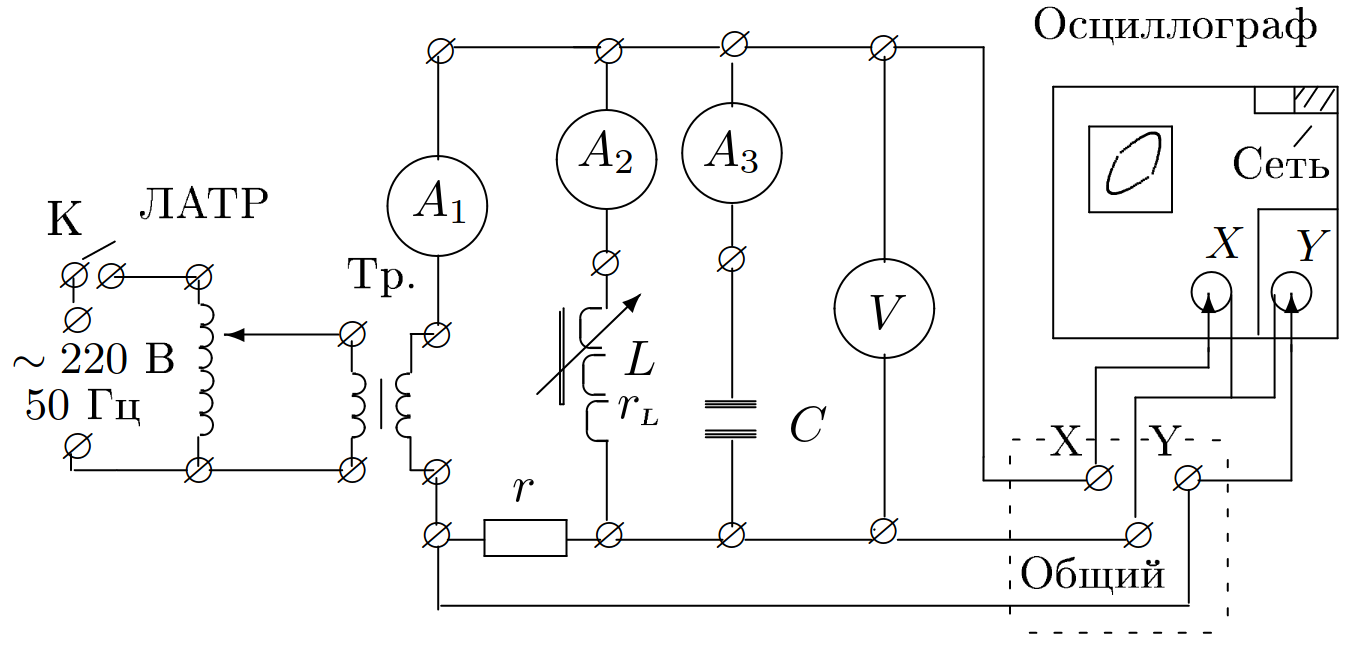
\includegraphics[scale = 0.2]{Workplace}
    \centering
    \caption{Схема установки}
\end{figure}

Напряжение от сети ($220$ В, $50$ Гц) с помощью ЛАТРа через понижающий трансформатор Тр подаётся на параллельный контур с конденсатором и катушкой, индуктивность которой зависит от глубины погружения сердечника. Параллельно с контуром включён реостат r.

Для наблюдения за сдвигом фаз между полным током и напряжением на контуре используется осциллограф. При наличии сдвига фаз между этими величинами на экране виден эллипс, а при нулевом сдвиге фаз эллипс вырождается в прямую.

\parag {Ход работы} ~\\

\point Соберём схему проверим её корректность. Подключим к сети, выставим необходимые значения.

\point Посмотрим, при каких положениях сердечника ток $I$ не превышает $0,5$ А. Получаем: $l_{min} = 35~мм$, $l_{max} = 115~мм$

\point Возьмём постоянное напряжение $U = 10~В$ и снимем значения токов $I$, $I_L$ и $I_C$ в зависимости от координаты сердечника $L$:

\begin{table}[!h]
    \begin{tabular}{|c|c|c|c|} \hline
        $L$, см & $I$, \% 0,5 A & $I_L$, \% 1 A & $I_C$, \% 1 A \\ \hline
        3 & 32 & 15 & 33\\ \hline
        3.5 & 28 & 20 & 34\\ \hline
        4 & 25 & 21 & 34\\ \hline
        4.5 & 21 & 23 & 34\\ \hline
        5 & 11 & 25 & 34\\ \hline
        5.5 & 8 & 27 & 34\\ \hline
        6 & 4 & 30 & 34\\ \hline
        6.5 & 3 & 33 & 34\\ \hline
        7 & 4 & 36 & 34\\ \hline
        7.5 & 10 & 39 & 34\\ \hline
        8 & 20 & 43 & 34\\ \hline
        8.5 & 27 & 47 & 35\\ \hline
        9 & 35 & 51 & 34\\ \hline
        9.5 & 45 & 56 & 35\\ \hline
        10 & 56 & 61 & 35\\ \hline
        10.5 & 67 & 67 & 34\\ \hline
        11 & 80 & 74 & 35\\ \hline
        11.5 & 96 & 81 & 35\\ \hline
    \end{tabular}
\end{table}

Построим график зависимостей токов от высоты сердечника:

\begin{figure}[!h]
    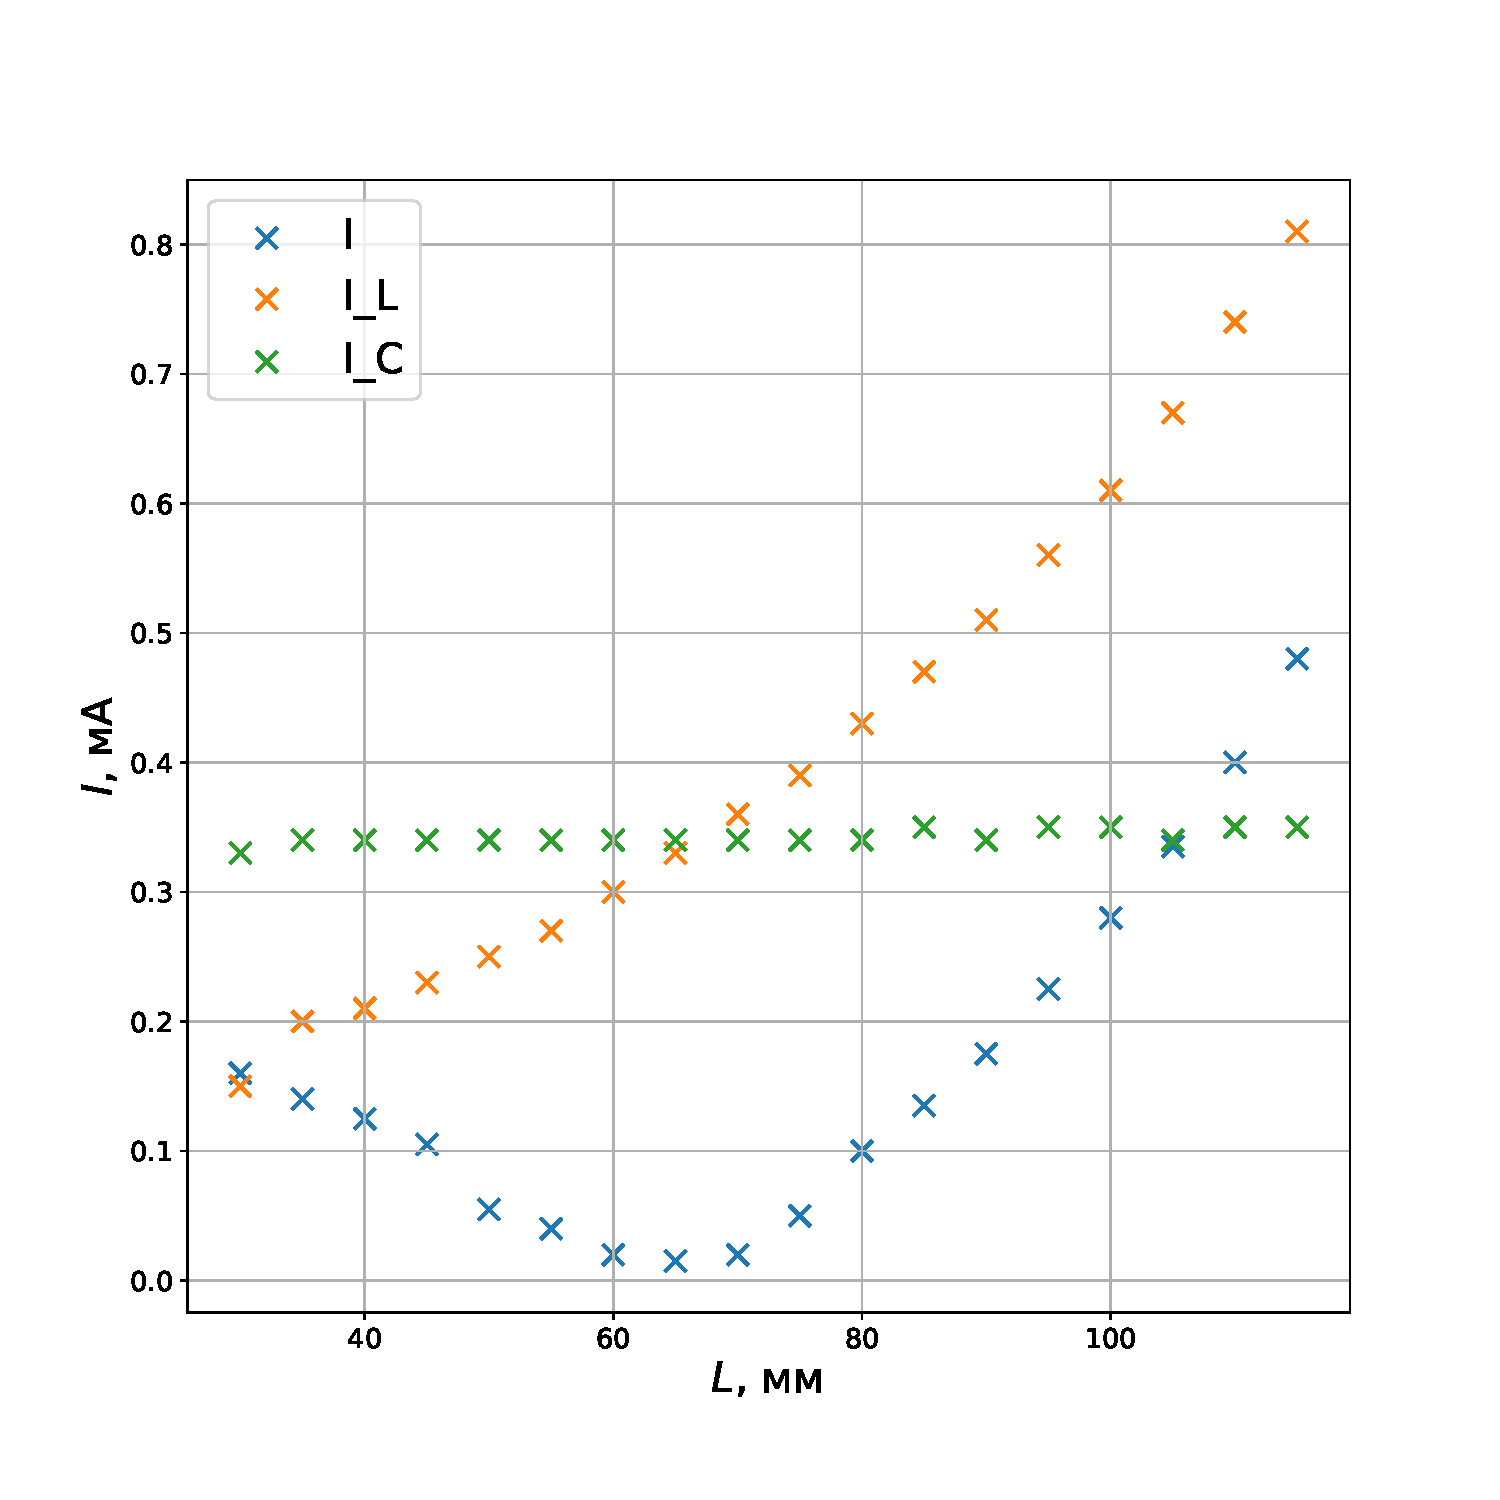
\includegraphics[scale = 0.5]{graph}
    \centering
    \caption{График $I (L)$}
\end{figure}

Заметим, что эллипс вырождается в прямую при $I = 15~мА$.

\point Вернём систему в положение резонанса и измерим токи. Получили: $I = 15~мA$, $I_L = I_C = 0,33~A$.

\point Оценим добротность и активное сопротивление катушки: $Q = 22$, $r_L = 4~Ом$ (значение измерено при $50$ Гц).

\parag {Обработка результатов} ~\\

Найдём добротность $Q$ и сопротивление при резонансе $R_{рез}$:

\[
    Q = \frac{I_{C-рез}}{I_{рез}} = \frac{I_{L-рез}}{I_{рез}} = 22 \pm 6
\]

\[
    R_{рез} = \frac{U_0}{I_{рез}} = 667 \pm 200 ~Ом
\]

\point Найдём индукцию $L_{рез}$ через ёмкость конденсатора $C$ и частоту $\omega_0 = 2 \cdot \pi \cdot \nu_0$ ($\nu_0 = 50 ~Гц$), а также $r_L$ через $C$ и $Q$:

\[
    L_{рез} = \frac{1}{\omega_0^2 \cdot C} \approx 0.08~Гн
\]

\[
    r_L = \frac{1}{\omega_0 \cdot C \cdot Q} = 1,2 \pm 0,4 ~Ом
\]

\point Теперь рассчитаем $L_{рез}$ через напряжение и силу тока на катушке:

\[
    L_{рез} = \frac{U_0}{2 \cdot \pi \cdot I_{L-рез}} \approx (9,0 \pm 0,3) \cdot 10^{-2} ~Гн
\]

\end {document}
